%%%%%%%%%%%%%%%%%%%%%%%%%%%%%%%%%%%%%%%%%
% Based on the "Masters/Doctoral Thesis" template (version 2.4) by:
% Steve Gunn (http://users.ecs.soton.ac.uk/srg/softwaretools/document/templates/)
% Sunil Patel (http://www.sunilpatel.co.uk/thesis-template/)
%
% Template license:
% CC BY-NC-SA 3.0 (http://creativecommons.org/licenses/by-nc-sa/3.0/)
%%%%%%%%%%%%%%%%%%%%%%%%%%%%%%%%%%%%%%%%%

%----------------------------------------------------------------------------------------
%	PACKAGES AND OTHER DOCUMENT CONFIGURATIONS
%----------------------------------------------------------------------------------------
\documentclass[
	11pt, % Default doc font size
	oneside, % Two side (alternating margins) for binding by default
	english, % Language
	singlespacing, % Single line spacing, alternatives: onehalfspacing or doublespacing
	%draft, % Uncomment for draft mode (no pictures, no links, overfull hboxes indicated)
	%nolistspacing, % If doc is onehalfspacing or doublespacing, uncomment to set spacing in lists to single
	%liststotoc, % Uncomment to add the list of figures/tables/etc to the table of contents
	%toctotoc, % Uncomment to add the main table of contents to the table of contents
	parskip, % Uncomment to add space between paragraphs
	%nohyperref, % Uncomment to not load the hyperref package
	headsepline, % Uncomment to get a line under the header
	chapterinoneline, % Uncomment to place the chapter title next to the number on one line
	consistentlayout, % Uncomment to change layout the declaration, abstract and acknowledgements pages to match the default layout
]{MastersDoctoralThesis} % Class file specifying document structure

\usepackage[utf8]{inputenc} % Required for inputting international characters
\usepackage[T1]{fontenc} % Output font encoding for international characters
\usepackage{tabularx}

\usepackage{palatino} % Use the Palatino font by default

\usepackage[backend=bibtex, style=trad-abbrv]{biblatex}
\setlength\bibitemsep{\baselineskip}
\addbibresource{References.bib}

\usepackage[autostyle=true]{csquotes} % Required to generate language-dependent quotes in bib

%----------------------------------------------------------------------------------------
%	MARGIN SETTINGS
%----------------------------------------------------------------------------------------
\geometry{
	paper=letterpaper, % letterpaper, a4paper, etc.
	inner=2.5cm, % Inner margin
	outer=3.8cm, % Outer margin
	bindingoffset=.5cm, % Binding offset
	top=1.5cm, % Top margin
	bottom=1.5cm, % Bottom margin
	%showframe, % Uncomment to show how the type block is set on the page
}

%----------------------------------------------------------------------------------------
%	THESIS INFORMATION
%----------------------------------------------------------------------------------------
\thesistitle{User Trust and Adherence toward Tiered Warning Messages in Web Browsers} % Use with \ttitle
\supervisor{Dr. Sonia \textsc{Chiasson}} % Use with \supname
\author{Matthew \textsc{Penny}} % Use with \authorname

\university{\href{http://www.carleton.ca}{Carleton University}} % Use with \univname
\department{\href{http://scs.carleton.ca}{School of Computer Science}} % Use with \deptname
\faculty{\href{http://science.carleton.ca}{Faculty of Science}} % Use with \facname
\degree{Bachelor of Computer Science} % Use with \degreename

% Set PDF metadata
\AtBeginDocument{
	\hypersetup{pdftitle={User Trust and Adherence toward Tiered Warning Messages in Web Browsers}}
	\hypersetup{pdfauthor=Matthew Penny}
	\hypersetup{pdfkeywords={Web security, usable security, HCI, warning messages, warning design}}
 	\hypersetup{linkcolor=black}
 	\hypersetup{citecolor=black}
}

% This report has "sections" not "chapters"
\makeatletter
\renewcommand{\@chapapp}{Section}
\makeatother
\begin{document}

\frontmatter % Use roman page numbering for pre-content pages
\pagestyle{plain} % Default to plain heading style until thesis style is called for body

%----------------------------------------------------------------------------------------
%	TITLE PAGE
%----------------------------------------------------------------------------------------
\begin{titlepage}
	\begin{center}
		\vspace*{.06\textheight}
		%{\scshape\LARGE \univname\par}\vspace{1.5cm}
		{\scshape\LARGE \href{http://www.carleton.ca}{
\includegraphics[scale=0.35]{Carleton-Logo}}\par}\vspace{1.5cm}
		\HRule \\[0.4cm]
		{\huge \bfseries \ttitle\par}\vspace{0.4cm}
		\HRule \\[1.5cm]
		\textsc{\Large Honours Project}\\[0.5cm]
 
		\begin{minipage}[t]{0.4\textwidth}
			\begin{flushleft} \large
				\emph{Author:}\\
				\href{http://www.mattp.ca}{\authorname}
			\end{flushleft}
		\end{minipage}
		\begin{minipage}[t]{0.4\textwidth}
			\begin{flushright} \large
				\emph{Supervisor:} \\
				\href{http://carleton.ca/scs/people/sonia-chiasson}{\supname}
			\end{flushright}
		\end{minipage}\\[3cm]
 
		\vfill
		COMP 4905\\\deptname\\[2cm]		
		\vfill
		{\large \today}\\[4cm]
		\vfill
	\end{center}
\end{titlepage}

%----------------------------------------------------------------------------------------
%	ABSTRACT PAGE
%----------------------------------------------------------------------------------------
\begin{abstract}
Users browsing the web frequently encounter warning messages in situations deemed dangerous by browser vendors. Current implementations use similar messages in all such cases, which could result in a greater likelihood of user habituation. We investigate the effectiveness of tiered warning messages of varying severity levels and appearances in an attempt to more strongly convey risk and thereby increase adherence rates.

We conducted a study in which 20 participants first reacted to an unanticipated warning message  and then, after learning the purpose of the study, 16 others. Most participants quickly ignored the warning in the first phase of the study, but in the second phase we found that our high severity tiered messages significantly outperformed the control messages in terms of user adherence and severity rating. Our low and medium severity tiered messages had significantly lower results in both areas. Additionally, users reacted more quickly to all tiered messages, on average, compared to the controls (whether dismissing them or adhering to them).
\end{abstract}

%----------------------------------------------------------------------------------------
%	ACKNOWLEDGEMENTS
%----------------------------------------------------------------------------------------
\begin{acknowledgements}
	\addchaptertocentry{\acknowledgementname}
	Thank you to my supervisor, \supname, for your consistent feedback and enthusiasm for discussion.
\end{acknowledgements}

%----------------------------------------------------------------------------------------
%	LIST OF CONTENTS/FIGURES/TABLES PAGES
%----------------------------------------------------------------------------------------
\tableofcontents
\listoffigures
\listoftables

%----------------------------------------------------------------------------------------
%	THESIS CONTENT - CHAPTERS
%----------------------------------------------------------------------------------------
\mainmatter % Begin numeric (1,2,3...) page numbering
\pagestyle{thesis} % Return the page headers back to the "thesis" style

\chapter{Introduction}
\label{Introduction}

Browsing the web entails many risks, and users are frequently faced with dangerous situations. It is important to make them aware of these dangers and reduce the likelihood of negative outcomes. In modern web browsers this is implemented in the form of warning messages which are presented to users in the event of suspected dangerous situations. However, research suggests that the existing messages and methods employed by browsers are not very effective and that users often ignore the warnings \cite{akhawe2013alice, almuhimedi2014reputation, anderson2015polymorphic, bravo2011bridging, dhamija2006phishing, egelman2008warned, sunshine2009crying}.

We believe that there is room for improvement in this area through more varied and easily understandable warning messages. In this study we experiment with the effectiveness of tiered warnings: messages which have varying severity levels and appearances depending on the situation in which they are triggered. We investigate how these new messages impact warning adherence and reaction time and which aspects of them influence user behaviour.

Our goal is to increase warning adherence by conveying the risk associated with dangerous situations more effectively. Conveying such information is difficult, particularly to users without a security background who simply want to browse the web. Common usability practices and past research in this area has shaped our warning message design in an attempt to learn from past mistakes, improve upon what works well, and incorporate new ideas.

\chapter{Background}
\label{Background}
There are many scenarios on the web which can result in the loss of user information or harm to the browsing device. These include phishing pages, pages infected with malware or other unwanted software, and the insecure transmission of sensitive information. Each of these scenarios can be dangerous for users and thus should generally be avoided.

Modern web browsers attempt to mitigate risk by displaying firm and assertive warning messages when a page is suspected to be dangerous (see figure \ref{fig:Warning-Firefox-SSL}). Unfortunately, many studies on the effectiveness of such messages have been conducted in the past and results have generally been poor. Users frequently ignore browser warnings and put themselves at risk nonetheless. Felt et al. \cite{felt2015improving} found that the rate of warning dismissal is 38\% in the case of Google Chrome’s SSL warning and in a study conducted by Sunshine et al. \cite{sunshine2009crying}., once participants learned how to ignore a warning in one situation, they typically ignored the warning in future encounters as well.

\begin{figure}[th]
	\centering
	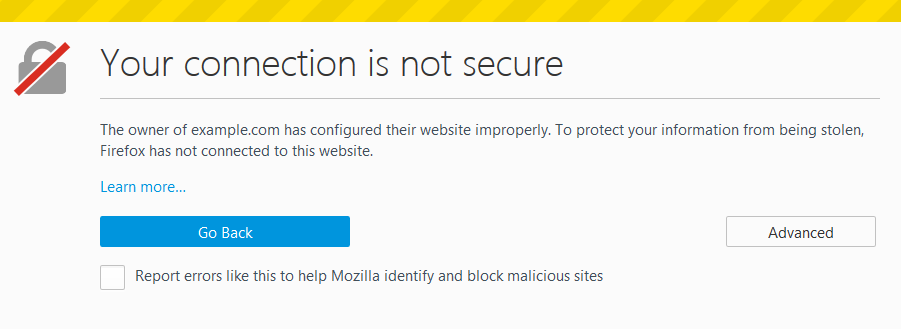
\includegraphics[width=\textwidth]{Figures/Warning-Firefox-SSL}
	\decoRule
	\caption[Firefox's SSL warning]{Firefox's SSL warning in Firefox version 52.}
	\label{fig:Warning-Firefox-SSL}
\end{figure}

Habituation is often identified by researchers as a critical reason for warning dismissal. \cite{akhawe2013alice, egelman2008warned}. Anderson et al. \cite{anderson2015polymorphic} investigated habituation at the neurological level and conducted a study which examined participants' brains in an fMRI machine while observing warning messages. They found that the effects of habituation could be seen after as few as two viewings of a given warning message. They were able to combat this phenomenon and significantly reduce the effects of habituation by using polymorphic, appearance-changing warning messages.

With this in mind, since similar looking warning messages are used in different situations, it is possible that the current approach to browser warning messages does not effectively convey important information. Understanding may instead be diluted by treating all warnings as equally severe. In this study, we investigate the impact of using tiered warning messages to alert users.

User understanding of risks is a key factor in adherence to warning messages. As has been found by Almuhimedi and Felt \cite{almuhimedi2014reputation} and Dhamija et al. \cite{dhamija2006phishing}, users generally ignore warnings because they do not understand the risks, or they trust the page they are attempting to visit and believe the warning was issued in error (i.e., a false positive). In the study conducted by Sunshine et al. \cite{sunshine2009crying}, some participants confused SSL warning messages with 404 pages, thinking that the server they were trying to access was down or somehow blocked. Thus, in addition to adherence rates, it is also of interest to know which \emph{aspects} (if any) of our tiered warning messages draw the attention of participants and if they truly understand the risks (not solely that any given warning as a whole is adhered to more or less frequently).

\chapter{Warning Message Design}
\label{Design}

This study involves participants reacting to different simulated warning messages of varying severity levels (mild, medium, and high severity) as well as the browser's default warnings as a control. We designed several warning messages for these conditions. The same warning structure is used in all cases, with warning content and style altered to reflect the risk of various simulated malicious situations. By experimenting with the severity levels (and thus the warning message features), we will examine how impressions and behaviour toward the different messages compare to one another.

The study aims to assess which aspects of warning messages more strongly convey severity and risk to users, and whether or not altering the expressed level of severity impacts user adherence (and by how much). As such, it is important to convey this notion of severity effectively through the messages' visuals so that users are able to quickly and intuitively distinguish between them -- even having never seen them before. Our warning messages utilize colour, wording, and imagery as cues for severity, which we hypothesize will increase understanding by maximizing the number of ways in which the danger level can be inferred.

\begin{figure}[th]
	\centering
	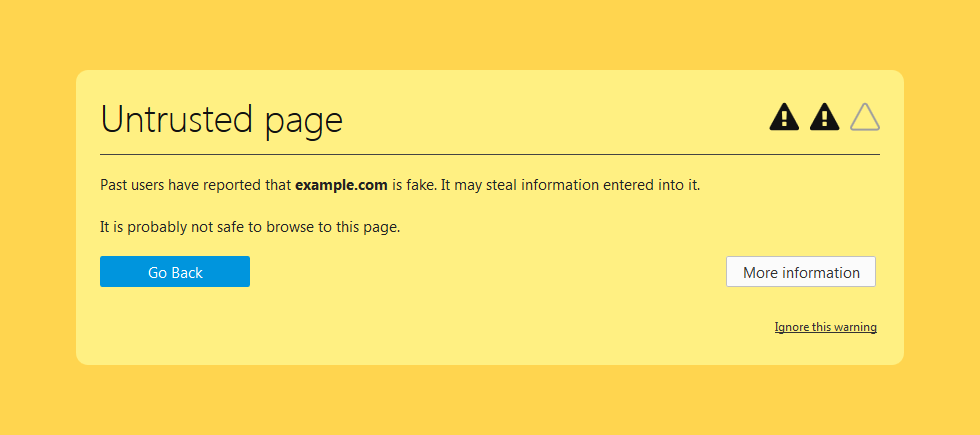
\includegraphics[width=\textwidth]{Figures/Warning-Medium-Phishing}
	\decoRule
	\caption[Medium severity phishing warning]{A medium severity phishing warning. Note the yellow colour, cautious wording, and two triangular icons. Colours, imagery, and wording are made more/less strict and intense as severity increases/decreases.}
	\label{fig:Warning-Medium-Phishing}
\end{figure}

\section{Colour}
Making colour the largest element is a reasonable design decision and is supported by research by Braun et al. \cite{braun1994color}, which indicates that colour plays an important role in warning adherence. In their study, participants complied with red warnings more frequently due to a higher associated likelihood of harm.

A message's colour covers the entire page, making it its largest, most obvious element. For our tiered warnings we chose to use colours with common real-world associations so their meanings would be intuitive, hopefully reducing the time and cognitive load needed to interpret the meaning of a given message.

Grey was chosen for low severity messages as it is usually considered neutral and is similar to the default background colour of a new tab in the browser. Yellow was used for medium severity messages due to its widespread association with ``caution'' (e.g., traffic lights, caution tape, construction). Red was employed in high severity messages because of its common link to stopping and danger (e.g., traffic lights, real-life warning signs, some existing browser warnings).

\section{Body Text}
Past studies have found that users are unlikely to read technical jargon or large amounts of text \cite{almuhimedi2014reputation, bravo2011bridging}. It is therefore important to convey a message's severity in an easy to understand manner while remaining concise. Our tiered warnings feature four main textual elements to accomplish this: the title, final note, threat explanation, and ``more information'' text.

\subsection{Title and Final Note}
The title and final note are modified based solely on a warning's severity (and not its type). They serve as global indicators of severity. The title of the warning aims to summarize the severity of the situation in two or three words. The final note serves as a cautionary message, further aiding in conveying the severity to the user by leaving them with some notion of how to proceed. See table \ref{tab:Tiered-Text} for these strings.

{\renewcommand{\arraystretch}{1.2}
\begin{table}[!htb]
	\small
	\centering
	\begin{tabularx}{0.85\textwidth}{|l|X|X|}
		\hline
		\textbf{Severity} & \textbf{Title} & \textbf{Final Note}\\
		\hline
		Low 	& Suspicious page 				& This page may be dangerous. Proceed with caution\\
		\hline
		Medium 	& Untrusted page 				& It is probably not safe to go to this page\\
		\hline
		High 	& Potential threat detected! 	& \textbf{It is highly recommended that you do not continue}\\
		\hline
	\end{tabularx}
	\caption{Tiered warning titles and final notes}
	\label{tab:Tiered-Text}
\end{table}}

\subsection{Threat Explanation}
Four different types of warnings were used for the study: SSL, malware, phishing, and unwanted software. For each type, a different group of threat descriptions was used. The purpose of this text is to emphasize the potential threat a user may be exposed to by visiting the page, as well as its impact. More stress and greater detail are given as the severity increases, with high severity warnings offering real-world examples of what can happen (e.g., passwords and financial information being stolen). The explanations are listed below in table \ref{tab:Tiered-Body}.

{\renewcommand{\arraystretch}{1.2}
\begin{table}[!htb]
	\small
	\centering
	\begin{tabularx}{\textwidth}{|l|X|X|X|X|}
		\hline
		\textbf{Severity} & \textbf{SSL} & \textbf{Malware} & \textbf{Phishing} & \textbf{Unwanted S/W}\\
		& \textbf{Warning} & \textbf{Warning} & \textbf{Warning} & \textbf{Warning}\\
		\hline
		Low
		& The authenticity of example.com, and thus its security, was unable to be verified.
		& example.com may contain software which can harm your computer.
		& The identity of the page at example.com, and thus the source of its contents, could not be verified.
		& example.com may contain potentially misleading and deceptive software\\
		\hline
		Medium
		& The identity of example.com could not be confirmed and therefore its security cannot be guaranteed. Information sent may be visible to others.
		& example.com may contain software which can harm your computer.
		& Past users have reported that example.com is fake. It may steal information entered into it.
		& Users have reported that example.com contains potentially unwanted software which it tries to install.\\
		\hline
		High
		& A secure connection could not be established to example.com. While browsing this website, it is possible for an attacker to monitor your activity and steal your personal information (passwords, financial information, conversations, etc.).
		& example.com has been reported by users in the past as being dangerous. It could contain malware.
		& example.com has been reported by users and it is likely impersonating another page. Any personal information entered (passwords, financial information, conversations, etc.) could be stolen.
		& example.com contains potentially dangerous and unwanted software which can negatively impact your computer. Users have reported that the page also employs trickery to encourage downloads of this software (e.g., fake download buttons).\\
		\hline
	\end{tabularx}
	\caption{Tiered explanations of threats}
	\label{tab:Tiered-Body}
\end{table}}

\subsection{``More Information'' Text}
It is presumed that users who click the ``more information'' button are seeking a detailed explanation. As such, the text revealed when the button is clicked is more verbose than the threat explanation, and remains the same for every tier of message of the same warning type (see table \ref{tab:Tiered-More-Info}). This always gives inquisitive users the level of detail they are seeking. The text is still relatively short and devoid of overly-technical wording.

{\renewcommand{\arraystretch}{1.2}
\begin{table}[!htb]
	\small
	\centering
	\begin{tabularx}{\textwidth}{|X|X|X|X|}
		\hline
		\textbf{SSL} & \textbf{Malware} & \textbf{Phishing} & \textbf{Unwanted S/W}\\
		\textbf{Information} & \textbf{Information} & \textbf{Information} & \textbf{Information}\\
		\hline
		Secure websites identify themselves using certificates. When a certificate is unable to be verified, it can mean that security settings have been misconfigured, security of the website has been compromised, or that an attacker is impersonating the website. In any case, any personal information entered into the page is at risk of being seen by others (e.g., passwords and credit card numbers).
		& Pages containing harmful software (malware) attempt to infect and take over your web browser and computer by installing malicious applications. Such software can allow attackers to steal personal information, delete files, and infect others.
		& Imitation pages impersonate sources you may trust and allow criminals to steal sensitive information such as passwords and credit card numbers. These pages may look and behave as expected, however information entered into them is actually sent to a criminal - not the organization the page claims to represent.
		& Unwanted software is classified as software that may behave in ways that you do not approve of or are not aware of. Examples include adware and spyware. Such software may also attempt to install additional unwanted software without your consent. Pages that distribute unwanted software often encourage downloads through deception (e.g., fake links, fake download buttons, and fake exit buttons).\\
		\hline
	\end{tabularx}
	\caption{Tiered warning ``more information'' text}
	\label{tab:Tiered-More-Info}
\end{table}}

\section{Imagery}
Our tiered messages feature a number of triangular ``warning'' icons alongside the title, with the number indicating severity (ranging from one icon for low severity to three icons for high severity). An example can be seen in figure \ref{fig:Warning-Medium-Phishing}. They are composed of an exclamation mark inside of a triangle -- an image often used on cautionary signs. The intent of this visual indicator is to provide a quick way for users to assess the severity of warnings. It is our hope that it will be useful in addition to the rest of the message, as well as on its own as a quick gauge of severity for users who do not read the message.

\chapter{Study Methodology}
\label{Methodology}

A tradeoff was made and the study was conducted in two phases in order to simultaneously gather more ecologically valid results as well maximize the amount of data collected. The first phase provided insight into participants' typical habits while the second gave more of an indication of their reasoning. The two phases correspond to our two areas of interest for the study: warning message adherence and captivating aspects of messages. An eye tracker was used for both phases of the study to determine where on the warning messages participants spent their time looking.

In short, participants were first exposed to one warning without any prior knowledge of the study. After learning the true purpose, we showed them all combinations of warning severity (low, medium, high, and control) and type (SSL, malware, phishing, and unwanted software) in a random order. We presented a two-question on-screen questionnaire after each message to measure risk perception and allow participants to explain their thought processes.

\section{Phase 1}
Participants did not initially know the true purpose of the study. In the first phase, they were told that we were investigating browsing habits and that they would be interacting with, reacting to, and giving feedback on various web pages. After calibrating the eye tracker, we pretended to have forgotten to show participants a particular form and asked to email it to them (for simplicity). It was mentioned that this was not mandatory, and an option was given to print the form instead if ``something went wrong'' or the participant felt uncomfortable logging in on a computer other than their own.

Upon navigating the web browser to the email login page, a warning message was triggered. Severity and type for this message was changed between participants. The software used to trigger the warning (detailed in section \ref{Methodology-Software}) noted whether or not participants ignored the message and tried to continue past to their email inbox as well as how long they spent making a decision. We then informed them of the true purpose of the study and clarified that there was no real threat and no data or information was at risk.

The goal of this phase is to obtain plausibly realistic results. This is encouraged in two ways. First, we suspect that participants will be more reluctant to ignore warning messages when their own personal information is supposedly at stake (e.g., their email login credentials and email messages themselves). Secondly, by being uninformed as to the study's true purpose, some bias will be removed. The behaviour will thereby more closely match that which would be observed in a non-laboratory environment.

\section{Phase 2}
The second phase involved participants reacting to various warning messages that they were presented with (either by clicking the ``go back'' or ``ignore'' button). The goal here is to obtain more data with regards to warning adherence, as well as to delve deeper into what makes a given warning worth paying attention to for participants. The tradeoff is that the data collected in this phase is less ecologically valid. Each participant was shown warnings of all types and severity levels mentioned above, with the ordering randomized.

In both phases of the study, the following questionnaire was displayed after each warning:

\begin{enumerate}
	\item How do you rate the severity of the warning message you just saw?
	\begin{center}
		\begin{tabular}{ccccc}
			Very low & Low & Medium & High & Very high\\
		\end{tabular}
	\end{center}
	\item Please explain the reason(s) for your answer to question 1 and choice to visit/not visit the fictional page.
\end{enumerate}


\section{Recruitment of Participants}
Participants for the study were recruited through social media, posters, and snowballing. An invitation to participate was posted on the researcher's Facebook page as well as a group page for individuals interested participating in studies at Carleton University. Posters using the same text as the social media invitation were also placed in typically busy locations around the Carleton University campus. In both of these cases, the study was described as being about web browsing habits so as to not compromise the deceptive aspect of the first phase. After completing the study, participants were encouraged to mention it to others (without divulging its true purpose and the deception employed in the first phase).

20 participants aged 18-57 took part in the study. All indicated on the demographic questionnaire that they browsed the web multiple times per day (10 on a mobile device and 10 on a PC). 10 participants were male, 9 were female, and one identified as genderfluid. Additionally, 7 of the participants indicated that they had a computer science background or had programmed before.


\section{Ethics}
Ethics approval for the study was obtained through Carleton University's Research Ethics Board prior to the recruitment of participants and the start of the study. Participants were each compensated \$10 CAD, regardless of whether or not they withdrew from the study.


\section{Software}
\label{Methodology-Software}
We developed a browser extension for Mozilla Firefox to display the different warning messages\footnote{See \url{http://github.com/mwpenny/warning-sim} for the source code.}. This approach was chosen so that messages could be shown in as realistic an environment as possible (i.e., within the browser itself, as opposed to static images). It also enables interactivity (e.g., the ``more information'' button can be clicked by curious users to reveal additional text describing the warning).

\begin{figure}[th]
	\centering
	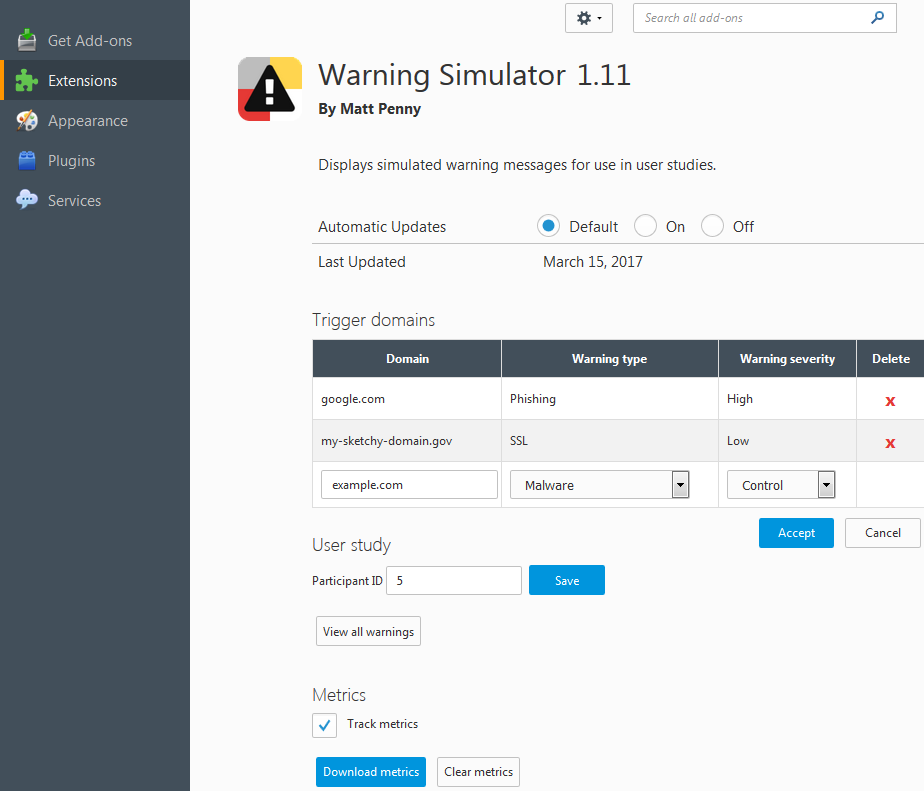
\includegraphics[width=0.925\textwidth]{Figures/Warning-Sim}
	\decoRule
	\caption[Warning simulator control panel]{The browser extension's configuration page. Experimenters can specify trigger domains, view all messages in a random order, and more.}
	\label{fig:Warning-Sim}
\end{figure}

Internal Firefox styling was also used to give the messages a look and feel similar to other ones users might have previously seen in the browser, adding to their authenticity. All of these factors result in a more realistic and authentic experience. Additionally, using web technologies to design the messages permitted quick and easy changes.

The extension allows an experimenter to specify a list of trigger domains for which warning messages should be displayed upon visiting (illustrated in figure \ref{fig:Warning-Sim}). For each domain, the warning type can be specified along with its severity. Alternately, a control message can be shown. This is useful for facilitating phase 1 of the study, in which unsuspecting participants are shown a warning message upon browsing to their email login page. There is also the ability to view all of the study's warning messages in a random order, one after the other -- enabling phase 2 of the study to be easily conducted.

The most obvious benefit of the browser extension is ease of data collection. Code was included to track which buttons were clicked and how much time was spent viewing a given warning before a decision was made, for example. The questionnaire mentioned above is also displayed after a warning's ``go back'' or ``ignore'' button is selected, easing the gathering of these responses for the two questions asked repeatedly throughout the study. All of this data is taggable with a configurable, anonymous participant ID and can be exported as a CSV spreadsheet.

Valuable data is also collected by the eye tracker, which records where participants look on screen and for how long. Visualizations such as heat maps and eye gaze trails can be superimposed over captured screen recordings. This information can be used to infer which aspects of the messages are most captivating to users.

\chapter{Results}
\label{Results}

We will first present our results pertaining to warning adherence by comparing user compliance for the control (Firefox default) warnings against our tiered messages. We will then delve into user understanding, making similar comparisons and examining reaction times and user ratings of warning severity.


\section{Warning Adherence}
\label{Warning Adherence}
\subsection{Control Warning Message Adherence}
The mean control warning message adherence rates for both phases of the study are summarized below in table \ref{tab:Adherence-Control}. For context, the number of participants for each value is also included. 

{\renewcommand{\arraystretch}{1.2}
\begin{table}[!htb]
	\small
	\centering
	\begin{tabularx}{0.85\textwidth}{|l|X|X|}
		\hline			
		\textbf{Warning Type} & \multicolumn{2}{|X|}{\textbf{Adherence Rate}}\\
		\cline{2-3}
		& \textbf{Phase 1} & \textbf{Phase 2}\\
		\hline
		SSL & 50\% (1/2) & 60\% (12/20)\\
		\hline
		Malware & 0\% (0/1) & 90\% (18/20)\\
		\hline
		Phishing & 100\% (1/1) & 80\% (16/20)\\
		\hline
		Unwanted Software & 100\% (1/1) & 85\% (17/20)\\
		\hline
	\end{tabularx}
	\caption{Control warning message adherence rates}
	\label{tab:Adherence-Control}
\end{table}}

With the exception of the malware warning in phase 1, the SSL warning had the lowest adherence rate. This is consistent with the findings of Felt et al. \cite{felt2015improving}.

\subsection{Tiered Warning Message Adherence}
The mean tiered warning message adherence rates for both phases of the study are summarized below in table \ref{tab:Adherence-Tiered}. For context, the number of participants for each value is also included.

{\renewcommand{\arraystretch}{1.2}
\begin{table}[!htb]
	\small
	\centering
	\begin{tabularx}{0.85\textwidth}{|l|l|X|X|}
		\hline
		\multicolumn{2}{|l|}{\textbf{Warning}} & \multicolumn{2}{|X|}{\textbf{Adherence Rate}}\\
		\hline
		\textbf{Type} & \textbf{Severity} & \textbf{Phase 1} & \textbf{Phase 2}\\
		\specialrule{.1em}{.0em}{.0em} 
		SSL & Low & 0\% (0/2) & 35\% (7/20)\\
		\cline{2-4}
		& Medium & 0\% (0/2) & 55\% (11/20)\\
		\cline{2-4}
		& High & 0\% (0/2) & 80\% (16/20)\\
		\specialrule{.1em}{.0em}{.0em} 
		Malware & Low & 100\% (1/1) & 45\% (9/20)\\
		\cline{2-4}
		& Medium & 0\% (0/1) & 65\% (13/20)\\
		\cline{2-4}
		& High & 100\% (1/1) & 100\% (20/20)\\
		\specialrule{.1em}{.0em}{.0em} 
		Phishing & Low & 100\% (1/1) & 45\% (9/20)\\
		\cline{2-4}
		& Medium & 100\% (1/1) & 65\% (13/20)\\
		\cline{2-4}
		& High & 100\% (1/1) & 95\% (19/20)\\
		\specialrule{.1em}{.0em}{.0em} 
		Unwanted S/W & Low & 0\% (0/1) & 45\% (9/20)\\
		\cline{2-4}
		& Medium & 0\% (0/1) & 65\% (13/20)\\
		\cline{2-4}
		& High & 0\% (0/1) & 75\% (15/20)\\
		\hline
	\end{tabularx}
	\caption{Tiered warning message adherence rates}
	\label{tab:Adherence-Tiered}
\end{table}}

In phase 1, all phishing and malware warnings (except for the medium severity malware warning) were adhered to every time. Every other type and severity of warning was ignored. In phase 2, adherence intuitively increases with severity for all message types (illustrated below in figure \ref{fig:Adherence-Tiered}).

\begin{figure}[!htb]
	\centering
	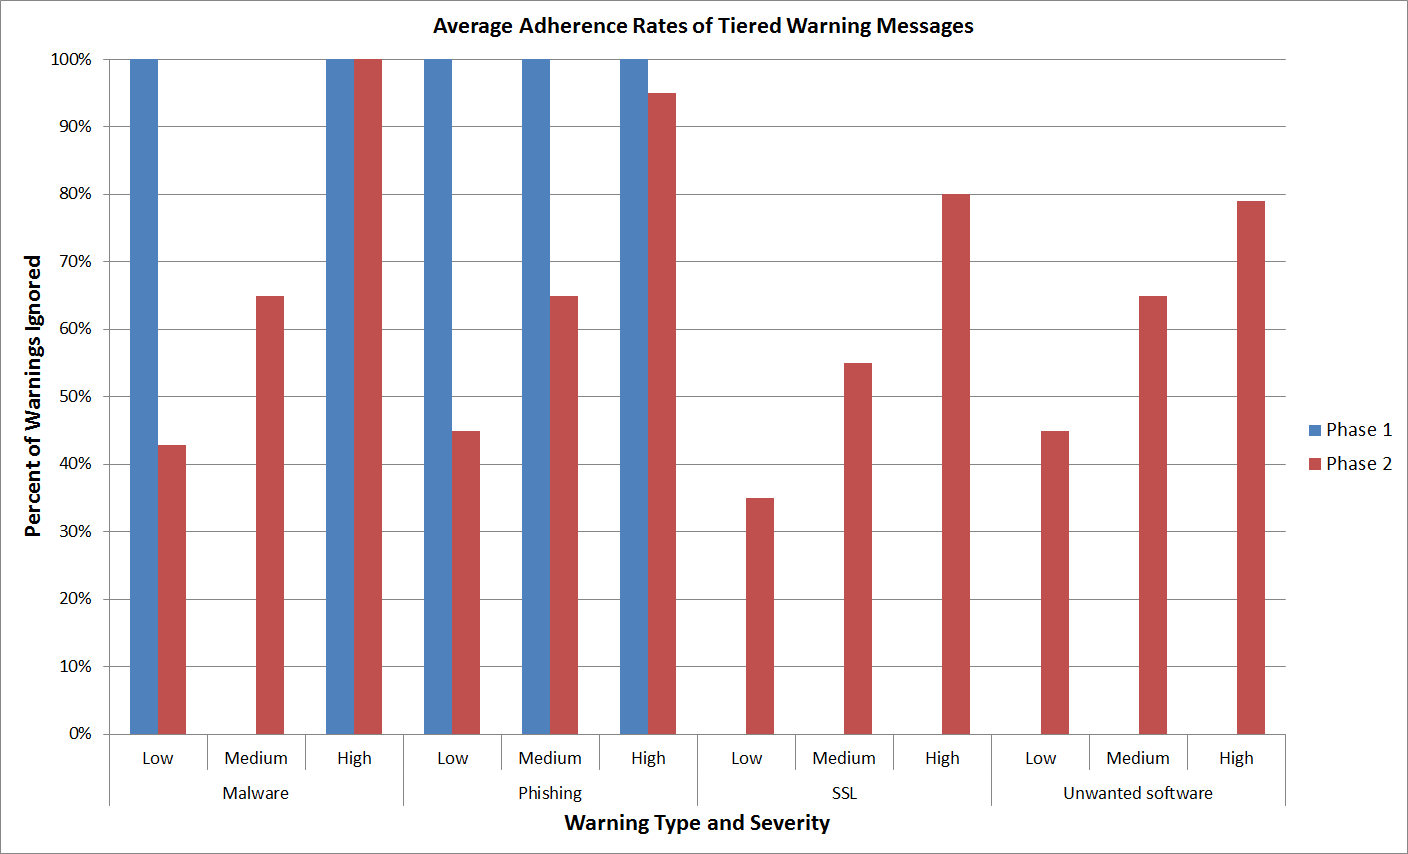
\includegraphics[width=\textwidth]{Figures/Adherence-Tiered}
	\decoRule
	\caption{Tiered warning message adherence rates}
	\label{fig:Adherence-Tiered}
\end{figure}

\subsection{Warning Message Adherence Analysis}
Six separate two-tailed t-tests were conducted. For each of the study phases, the mean adherence rate for the control warning messages was separately compared against the mean adherence rate for the low, medium, and high severity tiered messages.

In the first phase of the study, the mean adherence rate was always lower for the tiered messages than for the control ones. This difference was not found to be statistically significant.

In the second phase of the study, the mean adherence rates for the low and medium severity tiered warnings were lower than the control warnings (41.3\% and 62.5\%, respectively, versus 78.8\%). These differences in adherence rates were found to be statistically significant ($t(19) = 4.81, p = 0.0001$ in the the low severity versus control case and $t(19) = 2.94, p = 0.0084$ in the high severity versus control case).

The mean adherence rate in of the high severity tiered warnings in phase 2 was greater than that of the control warnings (88.8\% versus 78.8\%). This difference was found to be statistically significant ($t(19) = -2.37, p = 0.028$).

In summary, in phase 2, users were significantly more likely to adhere to our ``severe'' tiered messages and significantly less likely to adhere to our ``low'' and ``medium'' tiered messages, compared to the control messages.


\section{Reaction Time}
For each warning message presented in the study, our software measured the time that elapsed between when it was first shown and when participants made a decision (i.e., clicked either the ``ignore'' or ``go back'' button). For both the control and tiered messages, participants exhibited similar behaviour for decisions made within the first 20 seconds of being presented with a warning.

\subsection{Reaction Time for Control Warning Messages}
\begin{figure}[!htb]
	\centering
	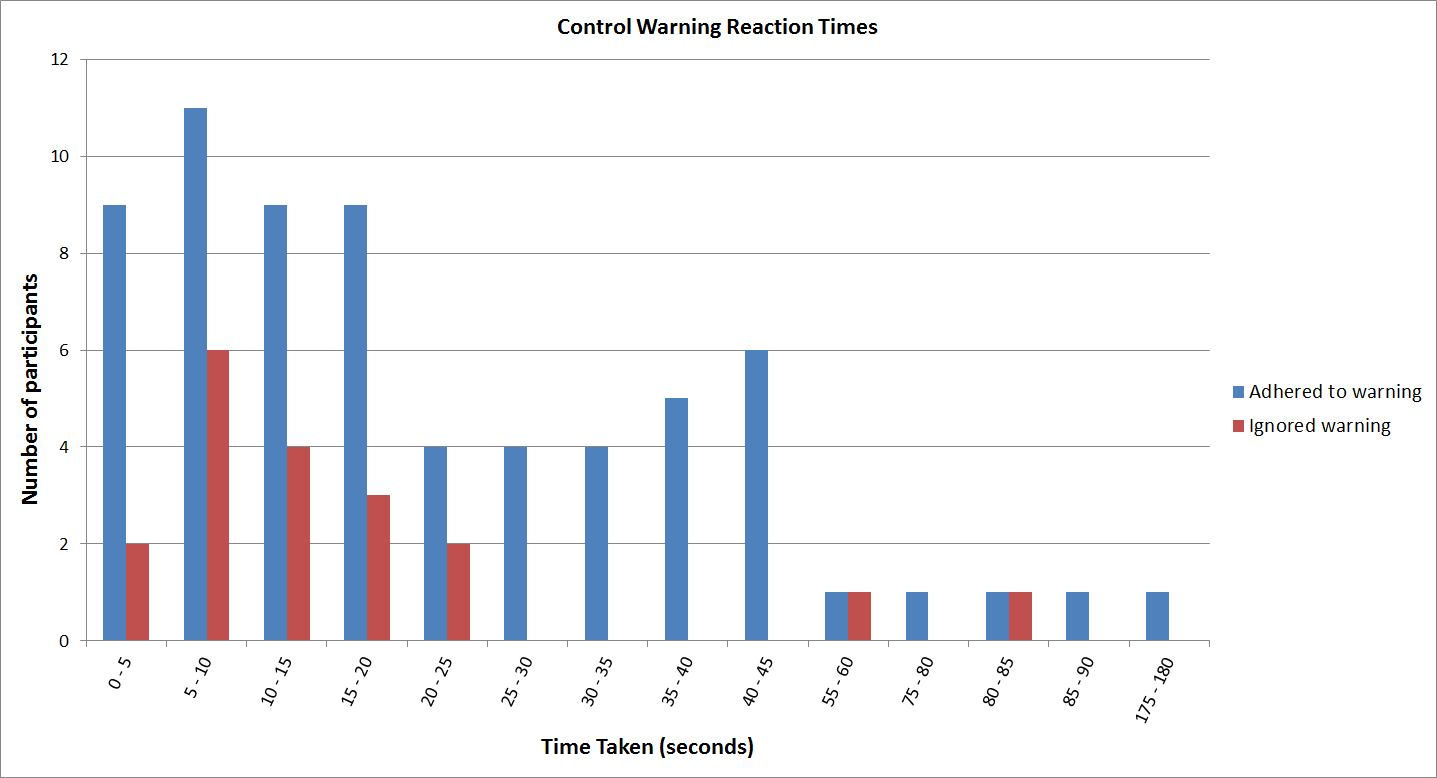
\includegraphics[width=\textwidth]{Figures/Time-Control}
	\decoRule
	\caption[Control warning decision times]{The amount of time taken by participants to make decisions regarding the control warning messages.}
	\label{fig:Time-Control}
\end{figure}
Most participants took between 5 and 10 seconds to make a decision after being faced with a control warning message (20\%). The rates of adherence and dismissal follow similar, bell curve-like distributions for relatively short times (below 20 seconds). For slightly longer times (between 20 and 45 seconds), adherence intuitively increases as the time spent observing the warning message increases. Additionally, dismissal in general does not occur as often beyond 20 seconds (only 12.5\% of the time). These results are illustrated in figure \ref{fig:Time-Control}.

\subsection{Reaction Time for Tiered Warning Messages}
These results are similar to those seen for the control warning messages. Again, most participants took between 5 and 10 seconds to make a decision (32.55\%). Unlike the control warnings, the majority of participants took less than 30 seconds to make a decision regarding the tiered messages (93.33\%). The rates of adherence and dismissal follow similar distributions: a steep increase before the 10 second mark and a decline afterwards. These results are illustrated in figure \ref{fig:Time-Tiered}.

\begin{figure}[!htb]
	\centering
	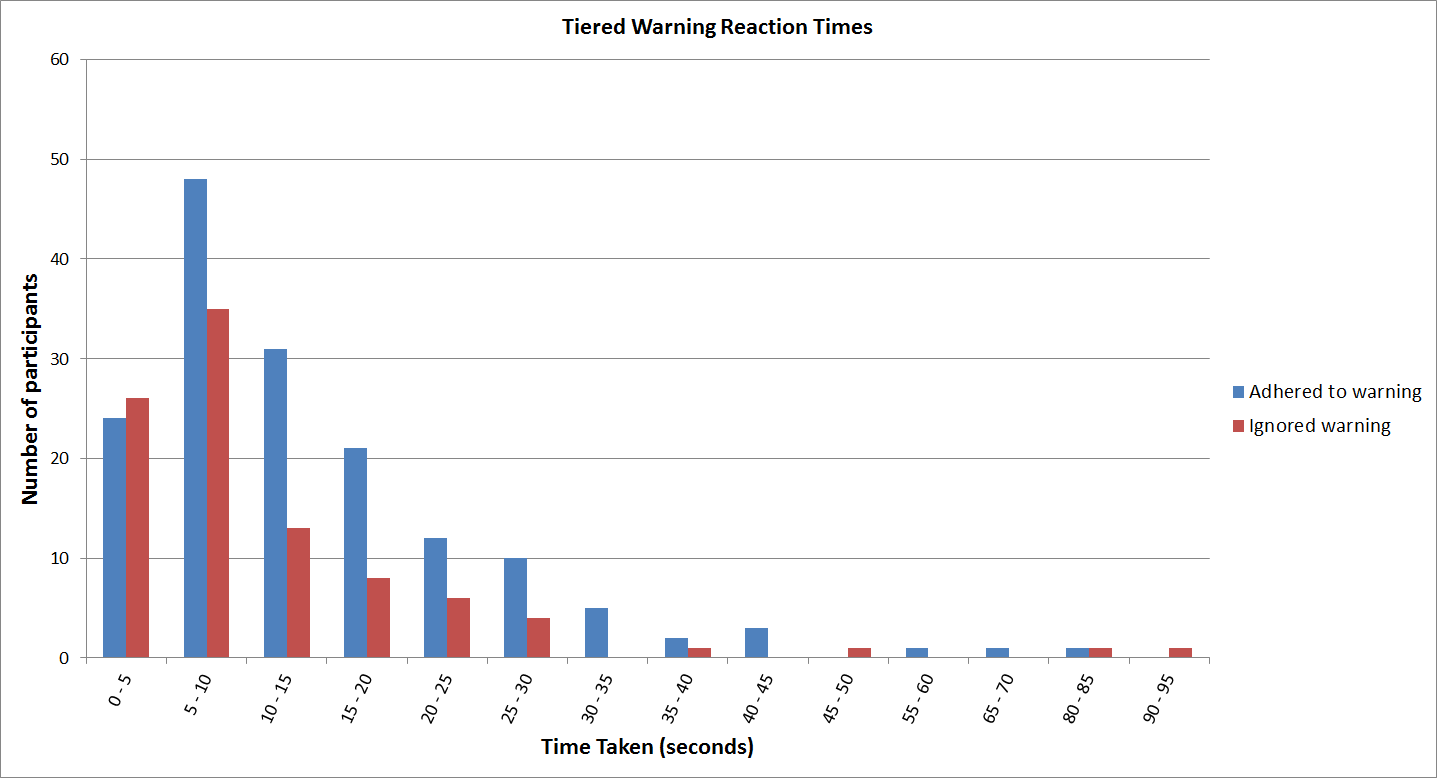
\includegraphics[width=\textwidth]{Figures/Time-Tiered}
	\decoRule
	\caption[Tiered warning decision times]{The amount of time taken by participants to make decisions regarding the tiered warning messages.}
	\label{fig:Time-Tiered}
\end{figure}

\subsection{Reaction Time Analysis}
The mean time taken to make a decision was compared between the control messages and the tiered messages in a two-tailed paired t-test. The average time was lower for the tiered messages than for the control messages (13.44 seconds versus 23.26 seconds, respectively) and the difference was found to be statistically significant ($t(19)=5.06, p=0.00007$).

This could mean that our tiered message express the warning content and severity more clearly to participants (making their decisions faster and easier), or alternately, that they come across as less important and are thereby more quickly dismissed. See section \ref{Discussion} for further discussion.


\section{Severity Rating}
For each warning message, participants were presented with an on-screen questionnaire after they chose to either adhere to or ignore it. The first question asked them to rate the message's severity on a 5-point Likert scale (with 0 being the least severe and 4 being the most severe). Consistent with the adherence rates in section \ref{Warning Adherence}, SSL ratings are generally rated the least severe.

\subsection{Control Warning Message Severity Ratings}
The average control warning message user severity ratings for both phases of the study are summarized below in table \ref{tab:Severity-Control}. For context, the number of participants for each value is also included. Participants generally chose higher ratings in phase 2, with the exception of the unwanted software warning.

{\renewcommand{\arraystretch}{1.2}
\begin{table}[!htb]
	\small
	\centering
	\begin{tabularx}{0.85\textwidth}{|l|X|X|}
		\hline			
		\textbf{Warning Type} & \multicolumn{2}{|X|}{\textbf{Severity Rating}}\\
		\cline{2-3}
		& \textbf{Phase 1} & \textbf{Phase 2}\\
		\hline
		SSL & 1.00 (2 participants) & 1.55 (20 participants)\\
		\hline
		Malware & 1.00 (1 participant) & 3.20 (20 participants)\\
		\hline
		Phishing & 2.00 (1 participant) & 3.00 (20 participants)\\
		\hline
		Unwanted Software & 4.00 (1 participant) & 3.05 (20 participants)\\
		\hline
	\end{tabularx}
	\caption{Control warning message severity ratings}
	\label{tab:Severity-Control}
\end{table}}

\subsection{Tiered Warning Message Severity Ratings}
The average tiered warning message user severity ratings for both phases of the study are summarized below in table \ref{tab:Severity-Tiered}. For context, the number of participants for each value is also included.

User severity ratings for low and medium tiered warnings were generally higher in the first phase of the study than the second. All high severity warnings were rated between 3 and 4 (between ``high'' and ``very high'' severity on our Likert scale) and all low severity ratings were rated between 0 and 2 (between ``very low'' and ``medium'' severity on our Likert scale). Additionally, the ratings in phase 2 of the study predictably increase with severity, similar to the adherence rates in section \ref{Warning Adherence} (illustrated below in figure \ref{fig:Severity-Tiered}).

{\renewcommand{\arraystretch}{1.2}
\begin{table}[!htb]
	\small
	\centering
	\begin{tabularx}{\textwidth}{|l|l|X|X|}
		\hline
		\multicolumn{2}{|l|}{\textbf{Warning}} & \multicolumn{2}{|X|}{\textbf{Severity Rating}}\\
		\hline
		\textbf{Type} & \textbf{Severity} & \textbf{Phase 1} & \textbf{Phase 2}\\
		\specialrule{.1em}{.0em}{.0em} 
		SSL & Low & 2.00 (2 participants) & 0.80 (20 participants)\\
		\cline{2-4}
		& Medium & 3.50 (2 participants) & 1.70 (20 participants)\\
		\cline{2-4}
		& High & 0.00 (2 participants) & 3.28 (20 participants)\\
		\specialrule{.1em}{.0em}{.0em} 
		Malware & Low & 2.00 (1 participant) & 1.19 (20 participants)\\
		\cline{2-4}
		& Medium & 2.00 (1 participant) & 1.84 (20 participants)\\
		\cline{2-4}
		& High & 2.00 (1 participant) & 3.50 (20 participants)\\
		\specialrule{.1em}{.0em}{.0em} 
		Phishing & Low & 1.00 (1 participant) & 0.85 (20 participants)\\
		\cline{2-4}
		& Medium & 1.00 (1 participant) & 1.80 (20 participants)\\
		\cline{2-4}
		& High & 2.00 (1 participant) & 3.50 (20 participants)\\
		\specialrule{.1em}{.0em}{.0em} 
		Unwanted S/W & Low & 1.00 (1 participant) & 1.00 (20 participants)\\
		\cline{2-4}
		& Medium & 1.00 (1 participant) & 1.85 (20 participants)\\
		\cline{2-4}
		& High & 1.00 (1 participant) & 3.00 (20 participants)\\
		\hline
	\end{tabularx}
	\caption{Tiered warning message severity ratings}
	\label{tab:Severity-Tiered}
\end{table}}

\begin{figure}[!htb]
	\centering
	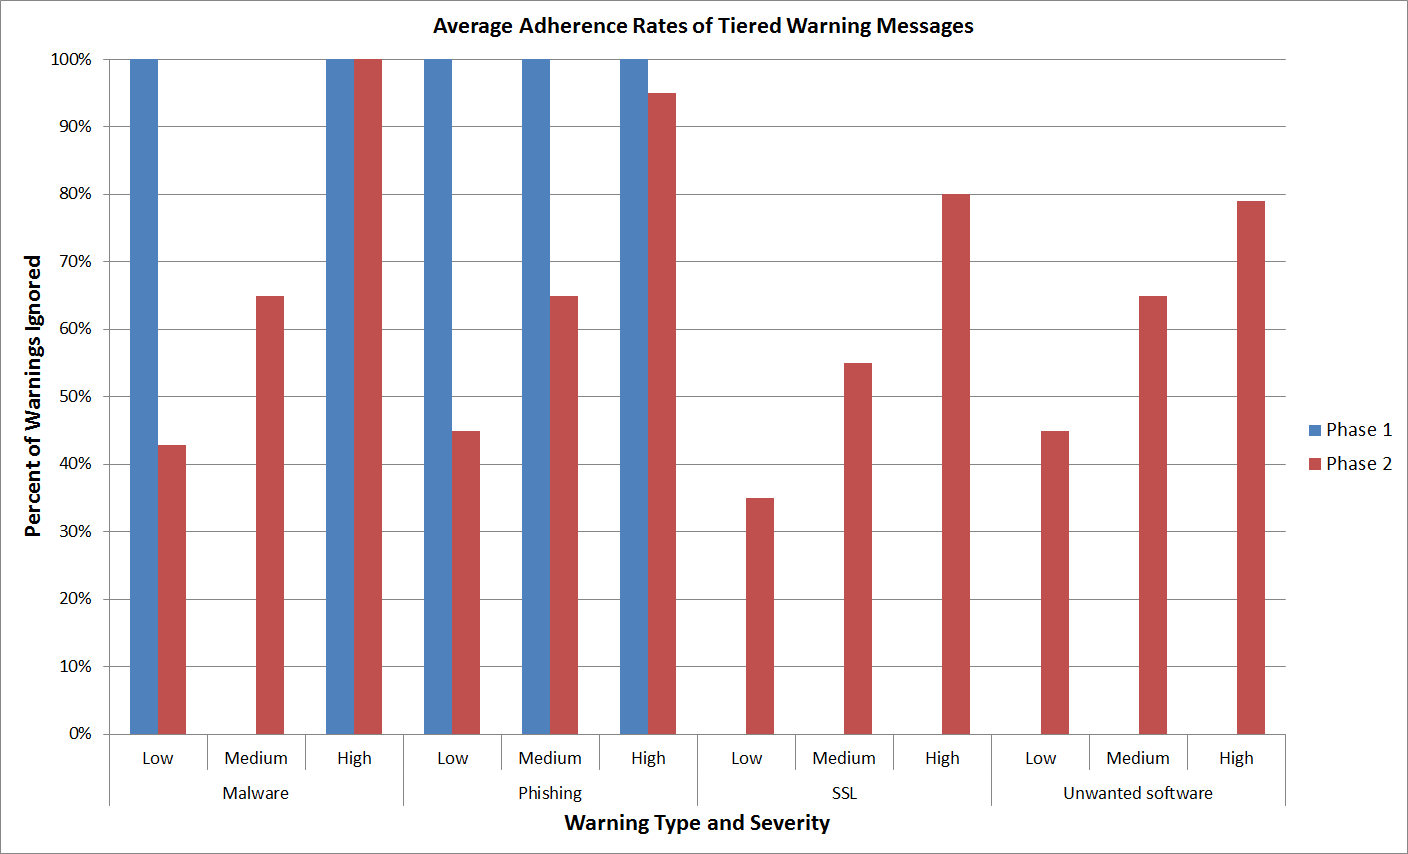
\includegraphics[width=\textwidth]{Figures/Adherence-Tiered}
	\decoRule
	\caption{User severity ratings for tiered warning messages}
	\label{fig:Severity-Tiered}
\end{figure}

\subsection{Severity Rating Analysis}
Six separate two-tailed t-tests were conducted. For each of the study phases, the mean user severity rating for the control warning messages was separately compared against the mean severity ratings for the low, medium, and high severity tiered messages.

In the first phase of the study, the mean user severity rating of the control messages was higher than the ratings of the low and high severity tiered warnings. However, this difference was not found to be statistically significant.

In the second phase of the study, the mean user severity rating was lower for the low and medium severity tiered messages when compared to the control messages (0.97 and 1.80, respectively, versus 2.70). In both cases, the difference was found to be statistically significant ($t(19) = 10.02, p = 5.09 \times 10^{-9}$ in the low severity versus control case and $t(19) = 6.03, p = 8.35 \times 10^{-6}$ in the medium severity versus control case). 

The mean user severity rating of the high severity tiered warnings in phase 2 was greater than that of the control warnings (3.30 versus 2.70). This difference was found to be statistically significant ($t(19) = -4.85, p = 0.0001$).

In summary, in phase 2, our ``severe'' tiered messages were rated as significantly more severe than the control messages by participants while our ``low'' and ``medium'' tiered messages were rated as significantly less severe than the control messages. This is consistent with the adherence rate findings in section \ref{Warning Adherence}.

\chapter{Discussion}
\label{Discussion}

In phase 2 of the study, we found that our high severity tiered warning messages outperformed Firefox's control warnings in terms of adherence rates, user reaction times, and user perceptions of severity. In this section, we will discuss possible reasons for these results, some other incidental findings from the study, and the overall implications.


\section{Phase 1}
Unfortunately, due to limited time and resources we were not able to collect enough data in phase 1 of the study to draw any statistically supported conclusions. Participants were debriefed after being presented with deceptive warning message. This means that each participant only saw one warning in this phase which consequently resulted in a very small sample size. However, behaviour during this phase should not be completely ignored as it provides some rough insight into user habits in a more ecologically valid scenario (no participants reported that they were aware of the deception used in phase 1). It also confirms the findings of previous studies.

Participants in phase 1 generally ignored the warning fairly quickly. Eye tracking data shows that many alternated between looking at the ``go back'' and ``ignore warning'' buttons repeatedly in apparent hesitation before making their final decision. It was also common for participants to fixate on a warning's title and skim or not read the body of the message (although some did). Both of these occurrences suggest to us that participants were trying to decide simply between visiting the website or not, rather than evaluating the type of risk the warning presented them with. The warning was merely acting as a roadblock in the way of their regular browsing -- a nuisance. Some expressed their disregard in the subsequent questionnaire with responses such as ``I didn't really pay attention to [the warning]'' and ``[The warning] was not difficult to read, but I should have read it slower''. This behaviour was seen for both the control messages and our tiered messages and is consistent with habituation effects and warning fatigue that have been previously observed by others \cite{akhawe2013alice, anderson2015polymorphic, egelman2008warned}.

\subsection{Perceived Risk}
We hypothesized that participants would be more likely to consider a warning message if they believed that personal information was at risk. We attempted to accomplish this in phase 1 by asking participants to sign into their university email account to view a form and triggering a warning when they attempted to do so. A real problem in these circumstances would jeopardize both login credentials and email messages themselves. Nevertheless, this scenario did not seem to have an effect on the participants. None which adhered to the warning cited a fear of stolen login credentials or email messages as their reason for doing so.

Although we informed participants that signing into their email accounts was optional, some noted that they felt it was necessary (e.g., ``I needed to go to my email so I was going [to the website] regardless''). This is likely due to a failure to convey the information, resulting in a misunderstanding. However, it is worrisome that, even in the face of severe warning messages, participants were willing forego security in the name of the study. Both of the above reactions suggest that the participants were not aware of the harm malicious websites can cause or that they do not care -- both of which are problematic. The latter was confirmed by one participant who told us ``[I] don't care about [the] security of Carleton email''.

\begin{figure}[!htb]
	\centering
	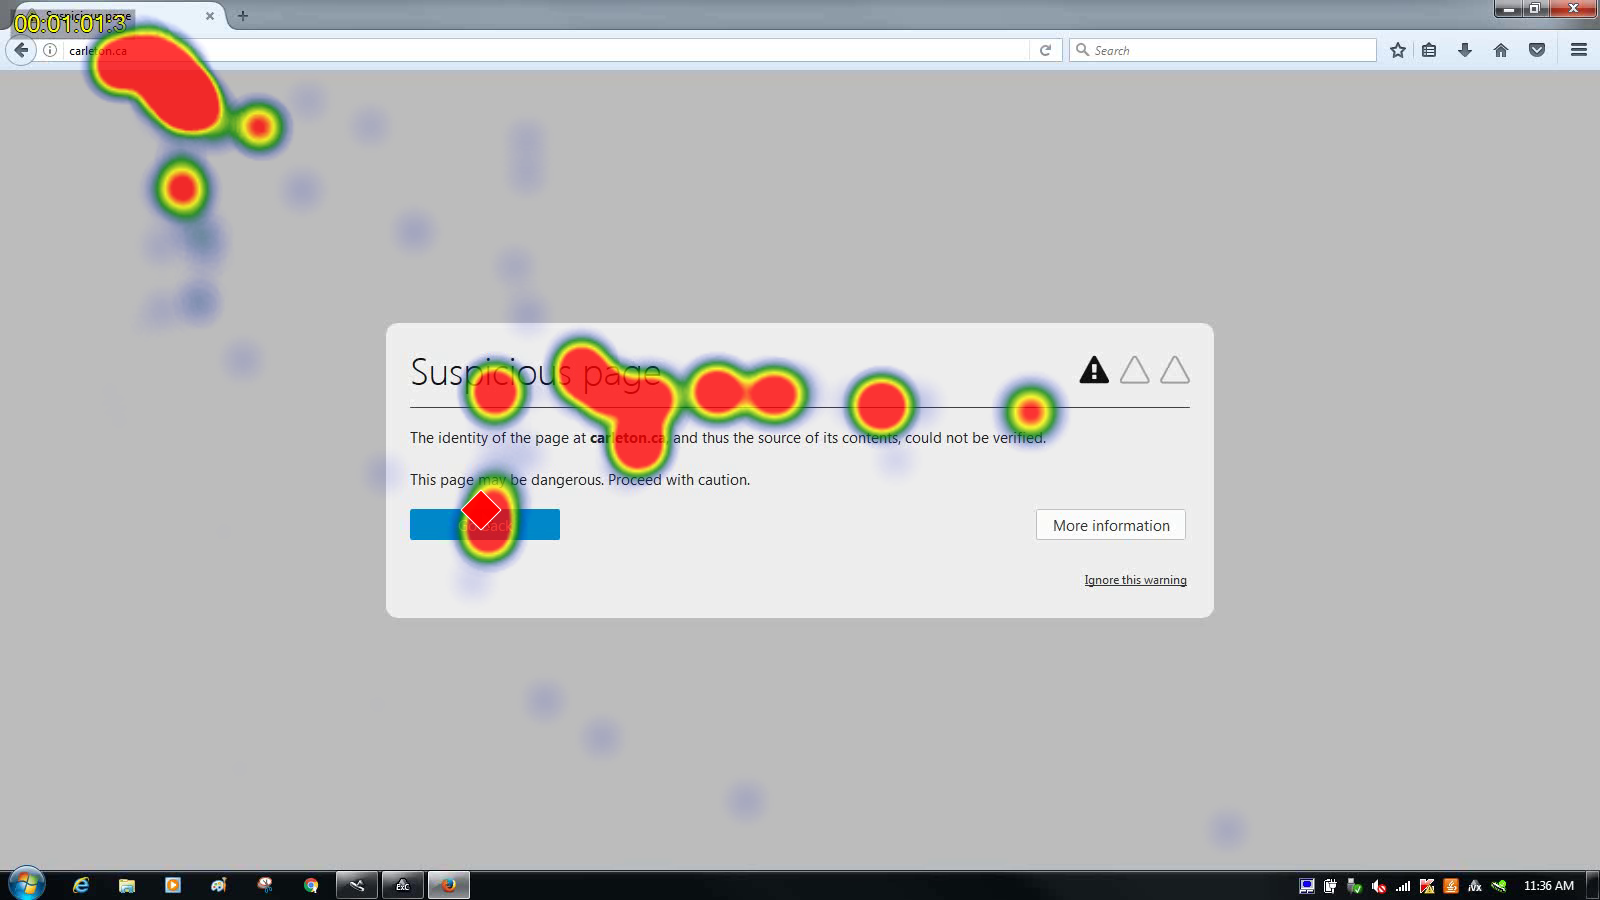
\includegraphics[width=\textwidth]{Figures/Heat-Map-P1-Low}
	\decoRule
	\caption[Phase 1 example heatmap]{A heat map of a participant viewing a low severity warning in phase 1 of the study. Note the focus on the title and lack of attention to the body. The participant also looked at the domain name (both in the URL bar and in the message body). The red diamond indicates a click.}
	\label{fig:Heatmap-Phase1}
\end{figure}

Eye tracking data shows that some participants checked the URL bar (presumably to verify that the destination URL was correct; a heatmap of one such instance is pictured in figure \ref{fig:Heatmap-Phase1}). This is typically a good security practice, but unfortunately a matching URL indicated total security for some. As Almuhimedi et al. \cite{almuhimedi2014reputation} found in a previous study, many participants trusted the website they were trying to visit and therefore felt it was probably still safe to continue regardless of the fact that a warning was displayed (e.g., ``I knew that the page was trustworthy'', ``Sometimes warning messages will appear on sites I know are safe/secure'', ``Ignored because I was accessing a trusted site''). Conversely, other participants understood that a warning on a trusted page is concerning, with remarks such as ``I was going to a page I've been to before so I automatically knew something was wrong'' and ``[An] email provider would never have such an issue so getting such a warning is very suspicious'', but these participants were in the minority. We attribute this divide in mindsets to a lack of (or improper) security education. The participants who trusted the email website appear to associate risk online purely with dangerous websites and do not consider the possibility of compromised servers (i.e., no harm can come when visiting a ``good'' website). Indeed, one participant stated that they had ``visited [the] webpage before without ill effects'', assuming that since nothing harmful had happened on the trusted site in the past, nothing harmful would happen in the future. There was little awareness of the fact that widely-used websites are large targets for attackers.

\subsection{Warning Comprehension}
Many participants ignored the warning in phase 1 relatively quickly. In a subsequent questionnaire, they were asked to identify the type of warning they had seen. Only participants who were exposed to an SSL certificate warning were able to recall it just moments later (with the exception of the low severity tiered warning). All other message types (malware, phishing, and unwanted software) could not be recalled, and many participants identified them as SSL certificate warnings as well. We suspect that most participants were guessing, with those in the SSL group happening to guess correctly. Again, this is consistent with habituation effects. Participants were likely over-exposed to SSL certificate warnings and consequently associated all browser warnings with certificate errors. Interestingly, at the conclusion of the study, all participants reported that the first message was either ``very easy'', ``easy'', or ``neutral'' in terms of clarity. We attribute this to faded memory and a lack of attention to the messages to begin with. 12 of our 20 participants changed their rating of the warning message in phase 1 when asked again at the conclusion of the study (after viewing all of the warnings in phase 2).


\section{Phase 2}

\subsection{Warning Adherence}
In phase 2 of the study we found that participants were significantly more likely to adhere to our high severity tiered messages and significantly less likely to adhere to our low and medium severity warnings (compared to the Firefox control warnings). This is explained by participants learning our warning cues over time. Eye tracker data shows that most participants initially looked at almost all aspects of the warnings but stopped reading the whole body of the messages (sometimes skimming it) after a while. A heatmap of one instance of this behaviour is pictured in figure \ref{fig:Heatmap-Phase2}. We observed a consistent pattern in the majority of participants: they would look at the warning title, then the imagery (if present), then the button corresponding to their decision, and finally they would click the button. They also began comparing warning messages to each other as the study went on. One noted that a low severity tiered warning ``only had one of three caution symbols filled in''. Another responded ``[This message is] not as intimidating as the red [one(s)]''.

Additionally, although every warning in phase 2 was unique (types did not repeat, severity levels did) many participants incorrectly stated at some point that they had seen a warning message previously in the study (e.g., ``I have already seen that warning multiple times and I have chosen to ignore it'', ``Repeated viewings of same warning, and I am ignoring them'', ``Same [warning] as before''). This behaviour indicates that they were only looking at warning features which changed with severity. Participants became habituated after learning the ``correct'' risk level and accompanying decision for a given warning tier. Those that ignored or adhered to a warning of a given severity level generally performed the same action for different messages of the same level, replicating the results of previous studies \cite{felt2015improving, sunshine2009crying}. 

\begin{figure}[!htb]
	\centering
	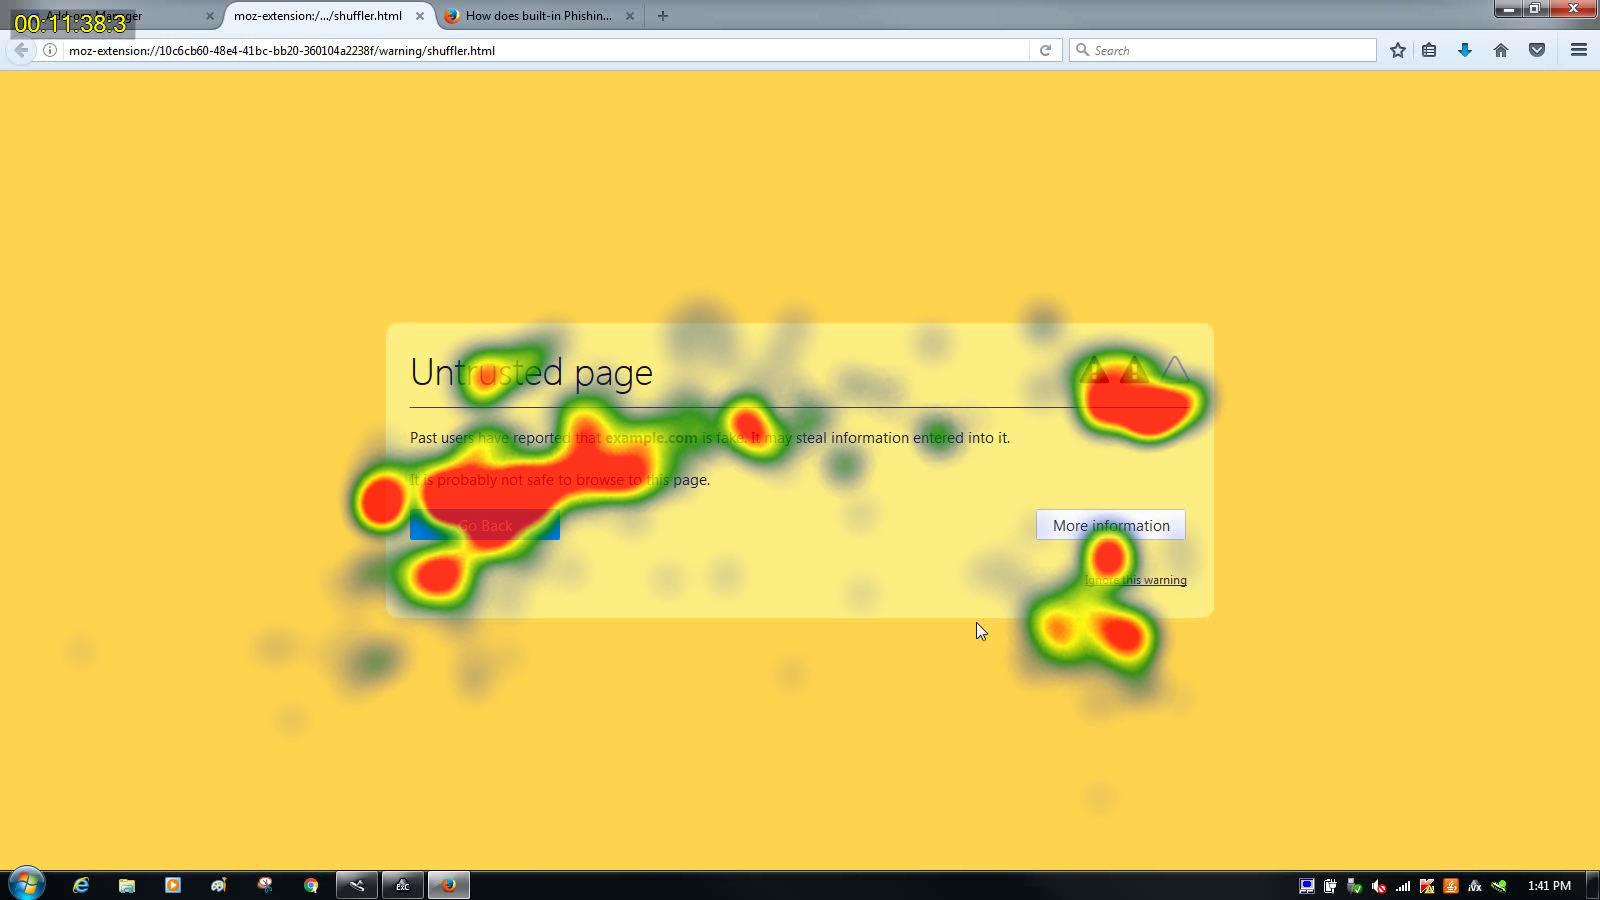
\includegraphics[width=\textwidth]{Figures/Heat-Map-P2-Medium}
	\decoRule
	\caption[Phase 2 example heatmap]{A heat map of a participant viewing a medium severity warning in phase 2 of the study. Note the attention paid to the warning icons and area surrounding the ``go back'' button.}
	\label{fig:Heatmap-Phase2}
\end{figure}

Participants had some other problematic ideas with regards to web security. For both the control and tiered warning messages, they vastly underestimated the difficulty in detecting and/or avoiding malware. Some participants who ignored warning messages responded that their reason for doing so was because they trusted either themselves or antivirus software to make the right decision with regards to security. For example, some responses to ignored ``unwanted software page'' warnings were ``I feel like the website is something my antivirus software can take care of'' and ``I [will] just make sure not to download anything and not to click suspicious-looking buttons''. Participants were unaware of attacks such as drive-by downloads and browser exploitation, which are admittedly unlikely to be known by the uninitiated.

\subsection{Severity Rating}
After learning our warning cues, participants consistently rated our high severity warnings as more severe than the control messages. We attribute this in part to a good warning design which allowed them to more easily gauge severity. As mentioned above, many participants compared our tiered messages to each other when explaining their perceptions of the severity.

The presence of the lower tiers of warnings likely also impacted severity ratings. Observing a high severity warning directly after a low severity one, for example, is a much more dramatic difference than seeing two consecutive high severity warnings. If true, this would mean that real-world users would need to be made aware of the other types of messages in order for high severity ones to be more effective. Unfortunately, the low and medium severity warnings had significantly \emph{lower} adherence rates than Firefox's default warnings. Adherence rates would have to be lowered in some cases in order to improve in others. A possible solution to this problem is to explain the different warning messages to users on first use of the browser and only show the lower tiers of messages when a threat is uncertain (a troubling tradeoff). On the other hand, it could be the case that the potential improved warning perception is not significant, and that the high severity warnings are effective on their own. However, this needs to be investigated further.

\subsection{Reaction Time}
Participants took significantly less time to make a decision when presented with a tiered message than they did with a control message. This is true for both warnings they ignored and those they adhered to. In section \ref{Results}, we suggested that this could mean either our messages conveyed severity in an easier to understand manner or that they appeared less important and were thereby more quickly dismissed. Given the improved results in adherence and severity perception, it is reasonable to conclude that the speed difference was due to a more easily identifiable level of danger.

\subsection{Warning Design}
\subsubsection{Colour}
Participant responses validated our assumptions about colour associations and our reliance on colour as a primary visual cue. On the post-study questionnaire, 80\% of participants rated colour as the most important factor for them in determining severity of messages (note that some participants tied colour with another feature of the messages). 18 of 20 rated red as the most severe colour, followed by yellow, and then grey. One rated yellow and grey as equal, and another rated grey as more severe than yellow due to a feeling of uncertainty. The responses are in line with our design goals and in phase 2 of the study our red messages were adhered to the most -- a result in agreement with the findings of Braun et al. \cite{braun1994color}.

\subsubsection{Body Text}
On the post-study questionnaire, 20\% of participants rated wording as the most important factor for them in determining severity of messages (note that some participants tied wording with another feature of the messages). Our severe messages featured concrete examples of real-world consequences such as passwords or financial information being stolen. Our goal was to make the harm more relatable and immanent, which participants picked up on (noting, for example ``I didn't like the possibility of other people seeing my passwords/private information'').

The threat description present in some of our tiered messages mentioned that other users had reported the fictional page. Participant reactions to these warnings were split. Some found the fact that another real human had reported the page more alarming, making the threat seem more legitimate. However, in others this resulted in a \emph{decreased} perception of the risk (e.g., ``It was reported to have security issues by other users, but not necessarily for me''). It is also possible that our brief (low severity) warnings caused participants to look into them more and be more cautious. One participant stated, ``somehow a more vague message made me more apprehensive than some of the others''.

At the conclusion of the study, the 20 participants were asked to identify all warning types which were presented to them in phase 2 from a list of possibilities (which included 4 warning types that were not present in the study). 15 participants remembered viewing SSL certificate warnings, 17 remembered malware warnings, 18 remembered phishing warnings, and 16 remembered unwanted software warnings. 6 participants chose one or more of the incorrect options. Although participants largely focused on the other aspects of the warnings, it appears that the body was succinct enough to effectively convey the warning type nevertheless in most cases.

\subsubsection{Imagery}
As mentioned above, eye tracking data shows that participants made frequent use of the triangular warning icons in assessing the danger of our tiered warning messages (e.g., some specifically cited low/high numbers of the icons for ignoring/adhering to a warning). Indeed, many were able to accurately describe the meaning of the imagery on the post-study questionnaire (e.g., ``More triangles meant it was more dangerous and risky to continue'', ``They were a rating system for the severity of the warning because they're similar to warning signs for the road'', ``The more icons there were the less likely I was to proceed with the page''). Additionally, one participant mentioned that they were dyslexic and that ``it was much easier to understand [the warnings] based on image and colour''. We therefore conclude that supplementing the other severity indicators with this information was very successful.

\pagebreak
\subsubsection{``More Information'' Text}
While not many participants clicked the ``more information'' button on our tiered warnings, those that did tended to read the entire threat explanation (shown in the eye tracking data). On the other hand, participants who clicked to find out more about a Firefox warning were discouraged. Doing so brought them to another page which contained information about 3 different types of warnings with no indication of which one the user came from. The approach taken by Mozilla proved to be very unusable. The page either confused participants or contained too much text to be deemed worth reading. Participants responded on the questionnaire that ``for the website to direct me to another website is kind of unusual to me'' and ``I didn't want to read the explicit explanation on the second page''. We suggest that warning designers provide a quick, clear, and easy way for users to find out more about the specific threat of interest without taking them out of current situation.


\section{Limitations}
As mentioned before, there were not enough participants to make statistically supported conclusions regarding the behaviour in phase 1 of the study. After viewing the first message, the surprise is ruined and therefore participants cannot be shown any more warnings. Possible solutions for this are to recruit more participants (if possible) or have participants perform benign tasks in between warning messages with the time between varying. The latter option, however, would be difficult to implement effectively without quickly alerting most participants to the true nature of the study. The data we did gather during phase 1 was nevertheless valuable for observing realistic behaviour and habituation effects, as well as reproducing the results of previous studies. Additionally, no participants claimed to be aware of the deception, meaning we were able to successfully structure the study so as to receive more genuine reactions.

Some participants in phase 1 noted that they felt they \emph{needed} to access their email inboxes when in fact we made a point to stress the opposite. According to these participants, having this mindset influenced their decision (it caused them to ignore the warning). In addition to the problem of few samples, this further taints our phase 1 data.

Another possible source of influence is the participants' awareness of the study's ethics approval. Participants might have assumed that their information was safe since the study was approved by the university's Research Ethics Board (noted on all recruitment material and the consent form). This would lessen any notion of risk in phase 1.

In phase 2 of the study, participants were fully aware of the purpose of the study and knew that they would be asked questions about the warning messages they were presented with. It is reasonable to assume that having this information in mind caused them to pay more attention to the warnings. The results obtained in phase 2 may therefore not be very generalizable to everyday browsing.

Next, as noted above, several participants' decisions in phase 2 were impacted by mention in some of the warning messages of other real-world users reporting danger. We did not explicitly plan the use of this wording other than purposefully excluding it from the low severity tiered messages. The presence of it in some messages at the medium and high tiers but not others may have affected participant behaviour and thus our results.

Finally, participants often compared our tiered warning messages to each other (e.g., ``there was only one warning symbol out of three that were coloured in'') and learned their relative severity ratings. Participants' perception of the high severity tiered message is likely predicated on the existence of the low and medium severity tiered warnings. Further experimentation is needed to determine whether or not the difference in perception of the high severity warning on its own is significant and how much it affects adherence.

\chapter{Conclusion}
\label{Conclusion}

In this study, we experimented with the use of tiered warning messages to convey risk to users while browsing the web. We found that our high severity tiered warnings had significantly higher adherence rates and user severity ratings compared to the warnings currently present in Firefox. Conversely, our low and medium severity tiered warnings had significantly lower adherence rates and user severity ratings. On average, participants reacted significantly more quickly to our tiered messages than the control messages (whether that decision was to adhere to a warning or ignore it).

Based on eye tracker data and participant responses, we attribute our results primarily to the use of colour and imagery in our warning messages. Participants were able to easily learn which messages were more severe using the provided cues and quickly make decisions when presented with new warnings of the same severity level. However, the learning was likely facilitated by the presence of the different tiers of warnings therefore it is questionable whether or not the high severity warnings would be as effective if they were presented on their own. Future research is therefore needed.

We suggest that warning message designers include multiple features to convey the risk of a given situation. For example, a dyslexic participant who had trouble reading the messages was able to quickly use colour and imagery instead. This redundancy aids in reinforcing messages and also catering to different users, making warnings more usable and accessable.


%----------------------------------------------------------------------------------------
%	BIBLIOGRAPHY
%----------------------------------------------------------------------------------------
\renewcommand\bibname{References}
\printbibliography[heading=bibintoc]

\end{document}  
